\documentclass[letterpaper, 10pt]{article}
\usepackage[activate={true,nocompatibility},final,tracking=true,kerning=true,spacing=true,factor=1100,stretch=10,shrink=10]{microtype}
\title{Protocolo de trabajo terminal}
\usepackage[document]{ragged2e}
\usepackage[spanish]{babel} %Indica que escribiremos en español
\usepackage[utf8]{inputenc} %Indica qué codificación se está usando ISO-8859-1(latín1)  o utf8  
\usepackage{amsmath} % Comandos extras para matemáticas (cajas para ecuaciones, etc)
\usepackage{amssymb} % Símbolos matemáticos (por lo tanto)
\usepackage{graphicx} % Incluir imágenes en LaTeX
\usepackage{color} % Para colorear texto
\usepackage{subfigure} % subfiguras
\usepackage{float} %Podemos usar el especificador [H] en las figuras para que se
% queden donde queramos
\usepackage{capt-of} % Permite usar etiquetas fuera de elementos flotantes
% (etiquetas de figuras)
\usepackage{sidecap} % Para poner el texto de las imágenes al lado
	\sidecaptionvpos{figure}{c} % Para que el texto se alineé al centro vertical
\usepackage{caption} % Para poder quitar numeración de figuras
\usepackage{commath} % funcionalidades extras para diferenciales, integrales,
% etc (\od, \dif, etc)
\usepackage{cancel} % para cancelar expresiones (\cancelto{0}{x})
\usepackage[table,xcdraw]{xcolor}
\usepackage{blindtext}
\usepackage{multicol} 

\usepackage{anysize} 					% Para personalizar el ancho de  los márgenes
\marginsize{2.54cm}{2.54cm}{2.54cm}{2.54cm} % Izquierda, derecha, arriba, abajo
\usepackage[colorlinks=true,plainpages=true,citecolor=blue,linkcolor=blue]{hyperref}
\usepackage{mathptmx}
\usepackage[T1]{fontenc}\usepackage{pslatex}

\usepackage{tcolorbox}
\tcbuselibrary{listingsutf8}
% Bibliografía

\usepackage[square,numbers]{natbib}
\renewcommand{\bibsection}{}
\bibliographystyle{unsrtnat}

% Tamaño de fuente
\newdimen\tamanyo
\newdimen\interlinea
\def\letra#1#2{%
\tamanyo=#1%
\interlinea=1.2\tamanyo%
\fontfamily{ptm}
\fontsize{\the\tamanyo}%
{\the\interlinea}\selectfont#2}

\hypersetup{
	pdftoolbar=true,        % show Acrobat’s toolbar?
	pdfmenubar=true,        % show Acrobat’s menu?
	pdffitwindow=false,     % window fit to page when opened
	pdfstartview={FitH},    % fits the width of the page to the window
	pdftitle={Sistema de predicción enfocado a procesos electorales con base en la socio-física},    % title
	pdfauthor={Josué David Hernandez Ramirez},     % author
	pdfsubject={TTR},   % subject of the document
	pdfcreator={Josué David Hernández Ramírez},   % creator of the document
	pdfproducer={XELATEX}, % producer of the document
	%pdfkeywords={análisis de imagenes} {glucometro} {glucosas} {aplicaciones m\'oviles} 
}


\begin{document}
\begin{center}
    \letra{14pt}{\textbf{Sistema computacional de predicción enfocado a procesos electorales con base en la socio-física}}\\
    \letra{12pt}{\textbf{\textit{Trabajo terminal No. -}}} \\
    \letra{12pt}{\textit{Alumno: Hernández Ramírez Josué David}} \\
    \letra{12pt}{\textit{Directores: Dr. Ramírez Díaz Mario Humberto, Dr. De Luna Caballero Roberto}} \\
    \letra{12pt}{\textcolor{black}{\textit{*email: \url{josuehernandezr1605@alumno.ipn.mx}}}}
\end{center}

\textbf{Resumen -} El presente trabajo terminal propone usar el enfoque socio físico para la predicción de resultados en los procesos electorales, teniendo como guía los trabajos de Galam.  Se realizará un sistema computacional que refleje los resultados teóricos propuestos por Galam enfocando los algoritmos socio físicos a este tema. El sistema computacional tiene como objetivo el calcular predicciones de procesos electorales usando formulas matemáticas y autómatas celulares.
\newline
\textbf{Palabras clave -} Física, Matemáticas, Minería de datos, Política, Socio-física, Autómata celular.

\section{Introducción}

La socio-físico es una nueva rama interdisciplinaria de la física que aboga por el uso de los métodos y conceptos de la física de sistemas complejos para el estudio de interacciones colectivas en sociedades y de los fenómenos sociales como propiedades emergentes de un conjunto de individuos. Serge Galam propone el uso de estructuras piramidales auto-dirigidas de abajo hacia arriba usando reglas de mayoría. \cite{MarioH.RamirezDiaz2014, Galam.1986, Galam1990, Galam1991, Galam2000}
\\
\vspace{5mm} %5mm vertical space
Con los conceptos que existen relacionados a la socio-física actualmente que cubren varios temas como: redes sociales, evolución de los lenguajes, dinamismo de la población, crecimiento epidemiológico, terrorismo, elecciones electorales entre otros, se desarrollará un sistema computacional enfocado a resolver el problemas de las elecciones electorales relacionados con el éxito o fracaso de estas.

\section{Objetivo}
Desarrollar un sistema computacional basado en el enfoque de socio-físico que permita realizar predicciones de resultados en los procesos electorales. 
%, estas predicciones están basadas en datos recolectados con el Programa de Resultados Electorales Preliminares de elecciones anteriores.

\section{Justificación}

La aplicación de la teoría de la socio-física y los modelos desarrollados por Serge Galam en el ámbito político de México ayudaría a tener predicciones con el enfoque de la socio-física y no solamente probabilísticos sobre las predicciones electorales con base a los datos recolectados de elecciones anteriores para estimar el grado de aceptación para un partido político determinado.
\\
\vspace{5mm} %5mm vertical space
Para los políticos puede proporcionar resultados estimados sobre la confiabilidad y aceptación en un proceso electoral mediante la socio-física y no solamente probabilísticos.

\section{Productos o Resultados esperados}
El producto final será:
\begin{itemize}
    \item Sistema computacional
    \item Manual de usuario
\end{itemize}

\section{Metodología}

Para este trabajo terminal se utilizará la metodología de desarrollo rápido de aplicaciones (DRA), dado que el tiempo de desarrollo es corto, esta metodología permite centrarse en el producto final, hace hincapié en el desarrollo de prioridades y la definición de los plazos de entrega, si estos empiezan a atrasarse permite la reducción de requisitos para el ajuste y de esta manera no aumentar la fecha limite de entrega. Por otro lado la participación de los usuarios es necesaria para el diseño del sistema.\cite{dra}
\begin{figure}[!ht]
    \centering
    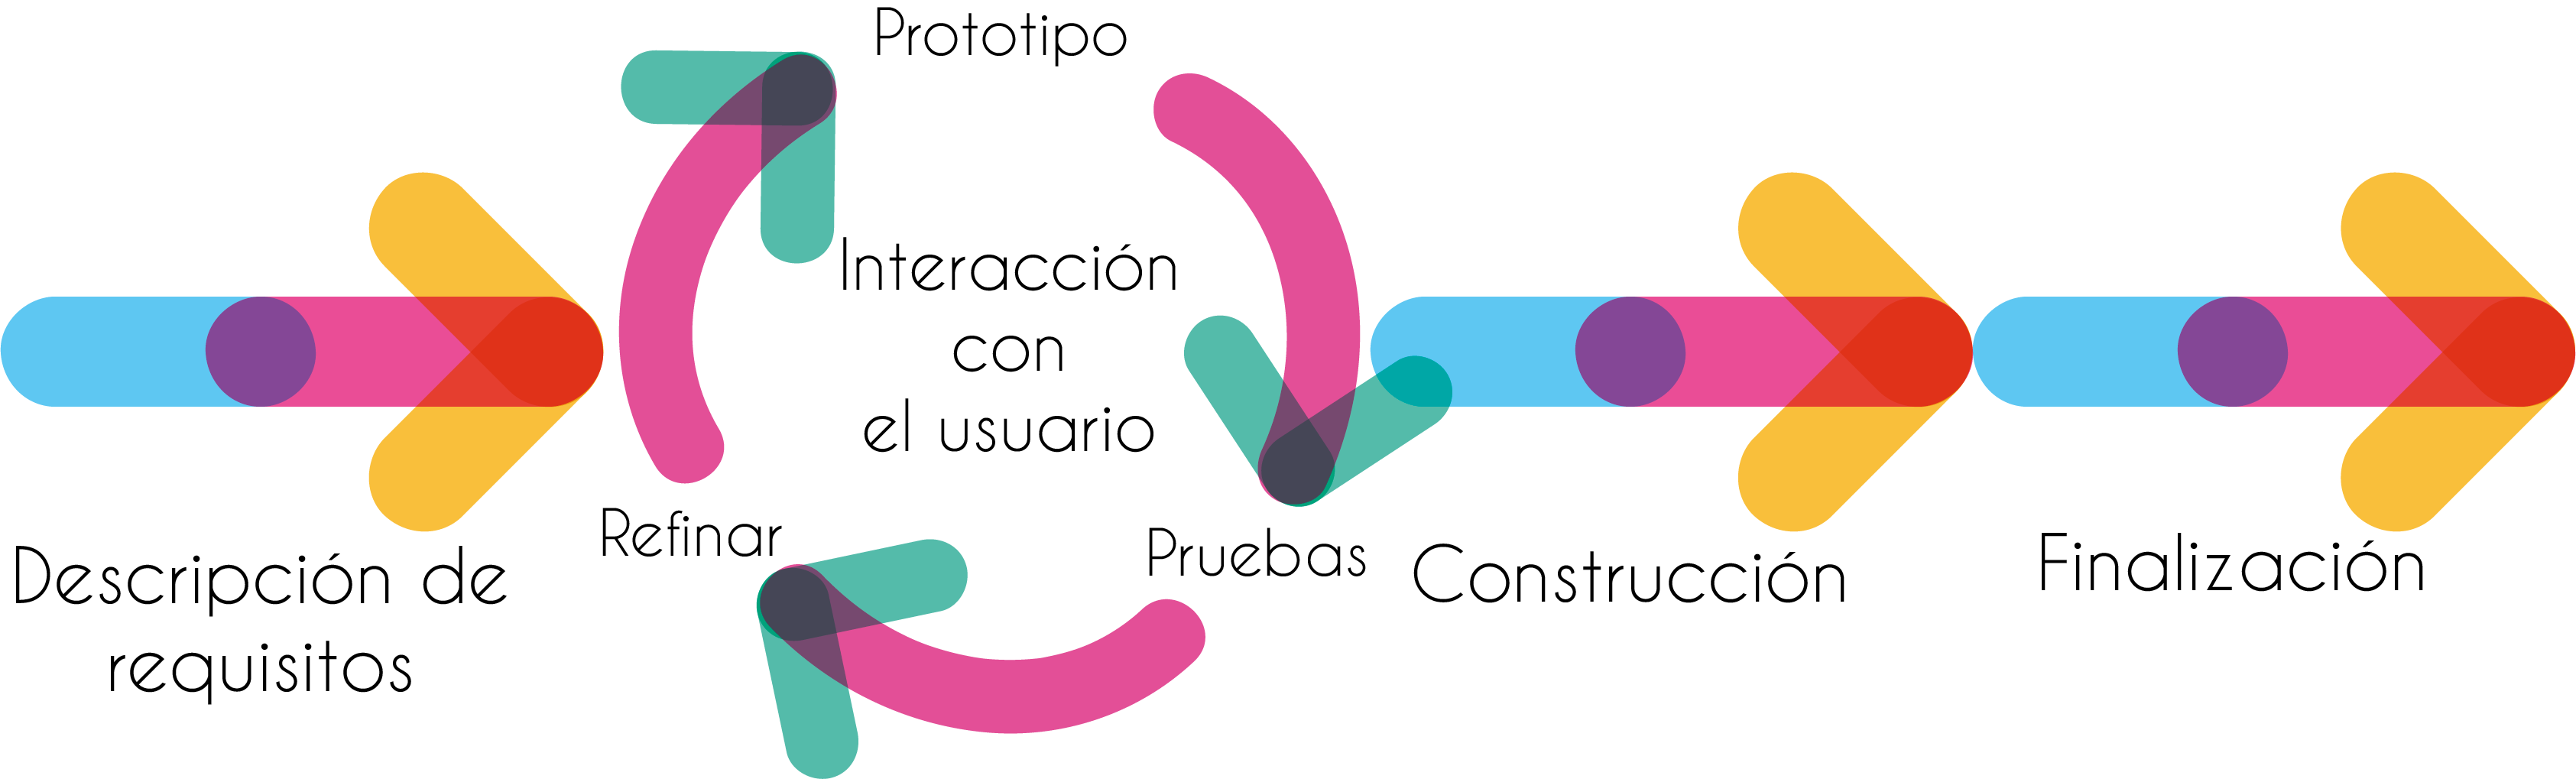
\includegraphics[scale=0.50]{Protocolo/images/4x/RAD@4x.png}
    \caption{Desarrollo rápido de aplicaciones}
    \label{graphic:PRecordatorio}
\end{figure}

\section{Cronograma}
\noindent
\textbf{Nombre del alumno:} \textit{Hernández Ramírez Josué David}\\
\textbf{Título del TT:} Sistema computacional de predicción enfocado a procesos electorales con base en la socio-física.
\begin{center}
    \begin{table}[!ht]
    \begin{tabular}{|p{11cm}|l|l|l|l|l|}
    \hline
    \rowcolor[HTML]{3531FF} 
    \multicolumn{1}{|c|}{\cellcolor[HTML]{3531FF}{\color[HTML]{FFFFFF} Actividad}} & \multicolumn{1}{c|}{\cellcolor[HTML]{3531FF}{\color[HTML]{FFFFFF} Ago}} & \multicolumn{1}{c|}{\cellcolor[HTML]{3531FF}{\color[HTML]{FFFFFF} Sep}} & \multicolumn{1}{c|}{\cellcolor[HTML]{3531FF}{\color[HTML]{FFFFFF} Oct}} & \multicolumn{1}{c|}{\cellcolor[HTML]{3531FF}{\color[HTML]{FFFFFF} Nov}} & \multicolumn{1}{c|}{\cellcolor[HTML]{3531FF}{\color[HTML]{FFFFFF} Dic}} \\ \hline
    Investigación sobre los principios y aplicaciones de la socio-física. & \cellcolor[HTML]{9B9B9B} &  &  &  &  \\ \hline
    Desarrollo del sistema basado en la socio-física para la predicción de las elecciones. & \cellcolor[HTML]{9B9B9B} & \cellcolor[HTML]{9B9B9B} & \cellcolor[HTML]{9B9B9B} &  &  \\ \hline
    Recopilación y análisis de datos para las pruebas del sistema. &  & \cellcolor[HTML]{9B9B9B} & \cellcolor[HTML]{9B9B9B} &  &  \\ \hline
    Ejecución de pruebas y ajustes del sistema. &  &  & \cellcolor[HTML]{9B9B9B} & \cellcolor[HTML]{9B9B9B} &  \\ \hline
    Prueba del sistema con datos reales. &  &  &  & \cellcolor[HTML]{9B9B9B} & \cellcolor[HTML]{9B9B9B} \\ \hline
    \end{tabular}
    \end{table}
\end{center}

\newpage

\section{Referencias}
\nocite{*}
\bibliography{bibliografia/bibliografia}

\newpage
\section{Alumno y directores}

\begin{multicols*}{2}
    \textit{Hernández Ramírez Josué David.- }Alumno de la carrera de Ingeniería en Sistemas Computacionales en la Escuela Superior de Cómputo, Especialidad Sistemas, Boleta: 2017630771, Tel. 7712413847, email \url{jhernandezr1605@alumno.ipn.mx}\\\\
    \vspace{5mm} %5mm vertical space
    \\
    Firma: \rule{7cm}{1pt}
    \vspace{5mm} %5mm vertical space
    \\
    \textit{Ramírez Díaz Mario Humberto.- }Doctor en Física Educativa, Maestro en Ciencias con Especialidad en Física y actualmente es profesor titular en el Departamento de Posgrado (Maestría en Ciencias en Física Educativa) del Centro de Investigación en Ciencia Aplicada y Tecnología Avanzada de Instituto Politécnico Nacional de México, Áreas de interés incluyen: socio-física, física educativa y epistemología de las ciencias, email \url{mramirezd@ipn.mx} \\ \\
    \vspace{5mm} %5mm vertical space
    \\
    Firma: \rule{7cm}{1pt}
    \vspace{5mm} %5mm vertical space
    \\
    \textit{De Luna Caballero Roberto.- }Licenciado en Ciencias de la Computación, Maestría en Tecnologías Educativas, Doctor en Educación, profesor de la Escuela Superior de Cómputo del Instituto Politécnico Nacional desde 1996, Áreas de interés incluyen: sistemas computacionales, algoritmos, estructura de datos, email \url{rdeluna@ipn.mx} \\ \\
    \vspace{5mm} %5mm vertical space
    \\
    Firma: \rule{7cm}{1pt}
    \vspace{5mm} %5mm vertical space
    \\
    \begin{tcolorbox}[colback=black!5!white,colframe=black!5!white,]
        \begin{flushright}
        \letra{8pt}{
            CARÁCTER: Confidencial
            \newline
            FUNDAMENTO LEGAL: Artículo 11 Fracc. V y Artículos
            108, 113 y 117 de la Ley Federal de Transparencia y Acceso
            a la Información Pública.
            \newline
            PARTES CONFIDENCIALES: Número de boleta y teléfono
        }
            
        \end{flushright}
   
    \end{tcolorbox}
    
\end{multicols*}

\end{document}